\clearpage
\section{Структура проекта}

\subsection{Контекст}
Контект является хранилищем для всех сущностей, представляющих какие-либо компоненты нейронной сети. Основной частью контекста является гетерогенный вектор - структура данных, хранящая все составляющие граф сущности. Для того, чтобы сущность могла быть сохранена в контексте, её класс должен быть унаследован от некоторого базового класса - это ограничение, накладываемое языком С++. В рамках контекста каждая сущность имеет уникальный идентификатор, однозначно определяющий её. Для того, чтобы скрыть часть интерфейса работы с такими сущностями и облегчить работу пользователя каждая сущность имеет разделение на имплементацию и обертку. Такое разделение идейно похоже на общеизвестную идиому Pimpl (pointer to implementation). 
\par
Кроме того, такой подход позволяет легче поддерживать динамическую обратную совместимость библиотеки. Динамическая обратная совместимость проявляется в следующем сценарии. Пользователь имеет приложение, к которому была прилинкована динамическая библиотека (.dll в ОС Windows, .so в ОС Linux). В случае выхода новой версии библиотеки при нарушении динамической обратной совместимости пользователь должен перекомпилировать свое приложение с новой библиотекой. Если же динамическая совместимость между версиями библиотеки не была нарушена пользователю достаточно лишь подменить библиотеку. Частой причиной нарушения этого является изменение порядка или состава членов классов, которые использует пользователь. Если пользователь скомпилирует свое приложение и будет взаимодействовать в нём лишь с обертками, то структура классов-имплементаций может быть изменена без нарушения динамической обратной совместимости.

\subsection{Тензор}
В общем случае тензор является N-мерной структурой хранения данных, таких как входные данные и параметры нейронной сети. В данный момент поддерживаются float и double типы данных для содержания их в тензоре.

\subsection{Операция}
Операция представляет собой абстракцию, которая инкапсулирует некоторую заданную её функциональность. Функциональная вершина графа может принимать объект операции и хранить его у себя. Это будет означать, что входящие в данную вершину соседи во время исполнения графа будут передавать свои результаты в аргументы операции, содержащейся в текущей вершине. Класс OperationInternal это базовый класс, являющийся по сути интерфейсом для всех реально применимых операций, таких как: сложение, умножение матриц, MSE. Основные методы этого интерфейса:
\begin{itemize} 
    \item Генерация кода, реализующего операцию.
    \item Генерация нового графа, представляющего собой производную от представляемой функции по $i$-му аргументу.
\end{itemize}
Удобство данного подхода заключается в том, что при создании новых операций достаточно выразить лишь первую их производную. Даже если в процессе работы будет требоваться производная $N$-го порядка, её без труда можно будет вычислить с помощью нового графа вычислений. Также можно не беспокоиться об уменьшении производительности из-за разворачивания сложных функций, поддерживаемых компьютером аппаратно, в граф вычислений - оптимизации на уровне генерируемого во время компиляции графа кода при возможности заменят последовательность простых функций на эквивалентную.
\par 
Помимо предоставляемых фреймворков операций пользователь сможет добавлять свои операции, что расширяет возможности применения фреймворка далеко за пределы искуственного интеллекта.

\subsection{Вершина}
Вершина представляет собой контейнер для действия над данными, будь-то их загрузка, преобразование или вывод пользователю.
\begin{figure}[ht]
    \centering
    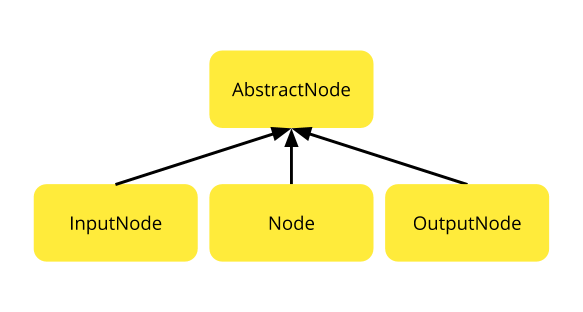
\includegraphics[width=0.8\linewidth]{NodeHierarchy.png}
    \caption{Иерархия классов вершин}
    \label{fig:nodes_hierarchy}
\end{figure}
Все типы вершин представлены иерархией классов, отображенной на рисунке \ref{fig:nodes_hierarchy}
\begin{itemize}
    \item \textbf{AbstractNode} -- абстрактный класс, инкапсулирующий общие для всех вершин поля: имя, число входящих рёбер, тензор результата.
    \item \textbf{InputNode} -- класс, позволяющий вносить данные в граф из различных хранилищ данных, а также хранить объект-загрузчик, необходимый для загрузки данных в граф из сторонних источников. Также может служить для хранения параметра графа вычислений, изменяющегося во время процесса оптимизации. 
    \item \textbf{Node} -- класс, позволяющий хранить объект операции.
    \item \textbf{OutputNode} -- класс, позволяющий хранить выдавать результат вычислений пользователю.
\end{itemize}

\subsection{Граф}
Граф представляет собой контейнер для набора ребер, описывающих топологию графа, а также множества индексов вершин, которые считаются начальными вершинами графа и будут задействованы первыми. Не требуется хранить индексы всех вершин графа явно, так как все вершины графа можно получить проходя из начальных вершин по ребрам. Кроме того граф хранит обход, о котором будет рассказано ниже.

\subsection{Резюме}
Для большего понимания можно взглянуть на рисунок \ref{Context}. На нем изображено как объект ContextInternal хранится внутри объекта Context, и при этом ContextInternal инкапсулирует в себе имплементации таких сущиностей как вершина, тензор и граф.
\begin{figure}[H]
    \centering
    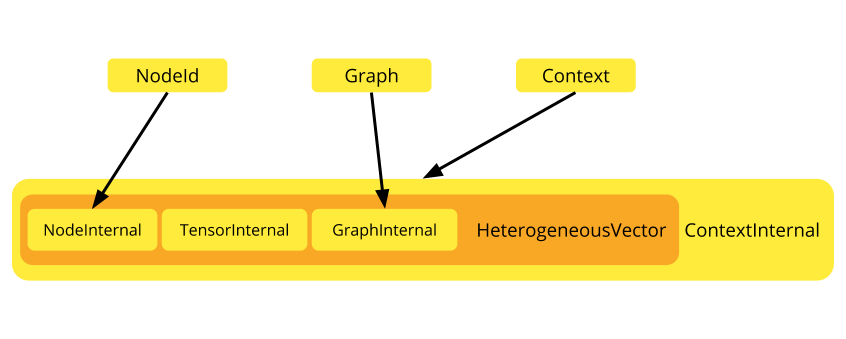
\includegraphics[width=0.8\textwidth]{Context}
    \caption{Расположение сущностей при проектировании графа.}
    \label{Context}
\end{figure}
В программном представлении работа по проектированию графа выглядит следующим образом.
\lstset{language=C++,
                keywordstyle=\color{blue},
                stringstyle=\color{red},
                commentstyle=\color{green},
                morecomment=[l][\color{magenta}]{\#}
}
\begin{lstlisting}[caption=Пример построения графа]
    auto graph = context.create<Graph>("mygraph");
    auto inp1 = graph.create<InputNode>(TensorShape{2, 2}, DataType::FLOAT, true, 0, "inp1");
    auto inp2 = graph.create<InputNode>(TensorShape{2, 2}, DataType::FLOAT, false, 0, "inp2");
    auto operationId = context.create<AddOperation>("myop");
    auto node = graph.create<Node>(operationId, "mynode");
    graph.connect(inp1, node, AddOperation::LEFT);
    graph.connect(inp2, node, AddOperation::RIGHT);
    auto out = graph.create<OutputNode>("out");
    graph.connect(node, out, Operation::Unmarked);
\end{lstlisting}
\par
С помощью технологии визуализации графов, предоставляемой \href{https://dreampuf.github.io/GraphvizOnline}{dreampuf.github.io}, такой граф можно представить так, как он выглядит на изображении \ref{GraphDotModel}
\begin{figure}[H]
    \centering
    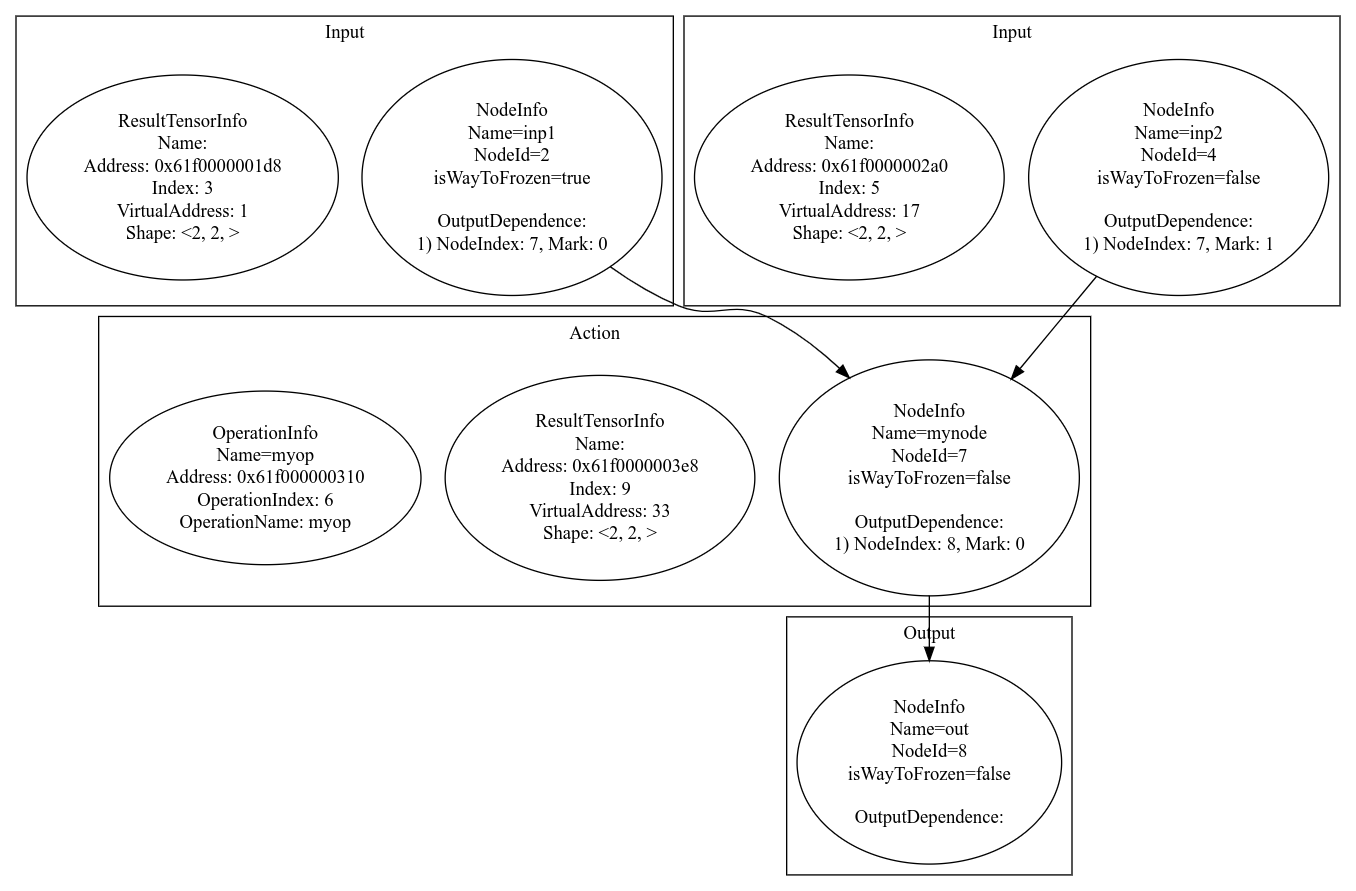
\includegraphics[width=0.8\textwidth]{GraphDotModel}
    \caption{Визуализация графа сложения.}
    \label{GraphDotModel}
\end{figure}